\documentclass[letterpaper,10pt,onecolumn]{IEEEtran}
\usepackage[margin=0.75in]{geometry}

\usepackage{graphicx}
\usepackage{amssymb}
\usepackage{amsmath}
\usepackage{amsthm}
\usepackage{cite}
\usepackage{alltt}
\usepackage{float}
\usepackage{color}
\usepackage{url}
\usepackage{titling}
\usepackage{balance}
\usepackage[subfigure]{tocloft} 
\usepackage{subfigure} 
\usepackage{enumitem}
\usepackage{pstricks, pst-node}
\usepackage{listings}
\usepackage{color}
\usepackage{tabularx}
\usepackage{textcomp}
\usepackage{pgfgantt}
\usepackage{hyperref}
\usepackage{changepage}
\renewcommand{\cftsecleader}{\cftdotfill{\cftdotsep}}

%% The following metadata will show up in the PDF properties
\def\name{Krisna Irawan\\ Jiongcheng Luo\\ Drew Hamm}
\def\doc{Technology Review}
\hypersetup{
  colorlinks = true,
  urlcolor = black,
  linkcolor  = black,
  pdfauthor = {\name},
  pdfkeywords = {capstone design, \doc},
  pdftitle = {\doc},
  pdfsubject = {\doc},
  pdfpagemode = UseNone
}

\begin{document}

\begin{titlepage}
	\centering
	{\scshape\LARGE Oregon State University\par}
	\vspace{2cm}
	{\huge\bfseries Head-Up Display Alignment System\par}
	\vspace{1cm}
	{\Large\bfseries \doc\par}
	\vspace{1cm}
	{\Large\itshape Senior Software Engineering Project (CS461)\par}
	{\Large\itshape Fall 2016\par}
	\vspace{1cm}
	{\normalsize\itshape Authors:\par}
	{\normalsize \name\par}
	\vspace{1cm}
	\vspace{3cm}


	% ============= Abstract =================
	\begin{abstract}
		This project is a proof concept to explore a potential technological innovation for Head-Up Display (HUD) system that present critical flight information to pilots. The primary objective of this project is to reduce the cost and time required to precisely align flight information to the HUD by introducing additional sensor to the system to make the alignment process more dynamic. To achieve this goal, there are nine different main technologies that will be critical for the development of the project. This document will compare three alternative options for each main technologies. This document will also include the option that we choose for each main technologies to develop this project. 

	\end{abstract}
\end{titlepage}
\tableofcontents

\newpage
% ============= Intro =================
\section{Introduction}
There are nine different main technologies that will be used or involved in this project. These technologies contain using of both software and hardware. For instance, for hardware, we will compare and discuss about some possible hardware options for building the demonstration system; for software, we will compare and discuss different algorithms or approaches for resolving the problem. Each of us takes an authorship (responsibility) for three technologies:\\

\textit{\textbf{Jiongcheng (Roger):}}
\begin{itemize}
	\item Hardware selection of Microcontroller
	\item Hardware selection of Represented MEMS IMU
	\item Hardware selection of Communication Protocol Type
\end{itemize}

\textit{\textbf{Krisna:}}
\begin{itemize}
	\item User Interface Toolkit
	\item Programming Language
	\item Statistical Analysis Method
\end{itemize}

\textit{\textbf{Drew:}}
\begin{itemize}
	\item IRU Data Representation
	\item Convert Raw MEMS Output to Quaternion Output
	\item Algorithm to get offset using both sensor outputs\\\\
\end{itemize}



% ============= content is put in individule file =================
\section{Technologies}
	

% ================================================================================================================================

\subsection{Hardware selection of Microcontroller}
\subsubsection{Context}
It is critical to choose the most appropriate microcontroller for this system since there are limitations from both hardware and software perspectives.
A microcontroller plays an important role in the system, which it will have following functionalities in the system:

\begin{itemize}
	\item Process input from the IMUs and output to the computer/display
	\item Process the alignment algorithm
	\item Debugging and testing purpose\\
\end{itemize}

\subsubsection{Options}
We consider to use a board between \textit{Adafruit Pro Mini}\cite{arduino}, \textit{Metro Mini 328}\cite{trinket} and \textit{InvenSense MPU-9250 CA-SDK Reference Board}\cite{MPU9250SDK}.
Anyone of these board has its outstanding areas and lack, and we will choose one of them based on the following criteria.\\

\subsubsection{Criteria}
\begin{enumerate}
	\item \textbf{Support Language}: We expect to use a general programming language for the microcontroller since using familiar programming language will reduce our time on additional research and the save time on working on the algorithm itself.
	\item \textbf{Clock Speed}: The alignment algorithm is required to within around 500 milliseconds time from taking the input from the IRUs to the output of aligned data, that require the board has a fast speed and running any processes.
	\item \textbf{I2C Protocol}: This is necessary to have on the board since the MPU-9250 (our selected IMU) require I2C protocol to communicate.
	\item \textbf{Connection with PC}: This is necessary to have on the board since we will use computer to any software program.
	\item \textbf{Size}: Size is less important since this system is for demonstration purpose.
	\item \textbf{Cost}: This is relatively important but as long as the price is within the expected budget, that will be acceptable.\\
\end{enumerate}

\newpage
\subsubsection{Table of Detailed Comparison}
\hfill \break
\begin{center}
\begin{tabular}{|c|c|c|c|}
\hline
\textbf{Model}                                                         & \textit{\begin{tabular}[c]{@{}c@{}}Arduino\\ Pro Mini\end{tabular}} & \textit{\begin{tabular}[c]{@{}c@{}}Metro\\ Mini 328\end{tabular}}          & \textit{\begin{tabular}[c]{@{}c@{}}InvenseSense\\ MPU-9250 CA-SDK Reference Board\end{tabular}} \\ \hline
\textbf{Core Chip}                                                     & ATmega328                                                           & ATmega328                                                                        & \begin{tabular}[c]{@{}c@{}}Texas\\ Instrument MSP430\end{tabular}                               \\ \hline
\textbf{Support Language}                                              & C                                                                   & C                                                                                & C/C++                                                                                           \\ \hline
\textbf{Clock Speed}                                                   & \begin{tabular}[c]{@{}c@{}}8MHz\\ (3.3V mode)\end{tabular}          & \begin{tabular}[c]{@{}c@{}}16MHz\\ (3V mode)\end{tabular}                        & \begin{tabular}[c]{@{}c@{}}16MHZ\\ (1.8V – 3.6V)\end{tabular}                                   \\ \hline
\textbf{\begin{tabular}[c]{@{}c@{}}I2C\\ Protocol/Number\end{tabular}} & Yes/1                                                               & Yes/1                                                                            & Embedded Structure                                                                              \\ \hline
\textbf{\begin{tabular}[c]{@{}c@{}}Connection\\ with PC\end{tabular}}  & USB                                                                 & FTDI/USB                                                                         & USB/Bluetooth                                                                                   \\ \hline
\textbf{Size}                                                          & 33mm x 18mm                                                         & 18mm x 44mm x 4mm                                                                & Unknown                                                                                         \\ \hline
\textbf{Cost (U.S Dollar)}                                             & \$9.95                                                              & \$12.50                                                                           & \$440.00                                                                                        \\ \hline
\textbf{Advantage}                                                     & \begin{tabular}[c]{@{}c@{}}Small\\ size\end{tabular}                & \begin{tabular}[c]{@{}c@{}}Faster\\ clock speed\end{tabular}                     & With embedded IMU                                                                               \\ \hline
\textbf{Shortage}                                                      & \begin{tabular}[c]{@{}c@{}}Slower\\ Clock Speed\end{tabular}        & \begin{tabular}[c]{@{}c@{}}Lack\\ of resource of guidance/datasheet\end{tabular} & High cost                                                                                       \\ \hline
\end{tabular}
\end{center}


\hfill \break
\subsubsection{Overall Discussion}
By comparing these boards by the above criteria, \textit{Arduino Pro Mini} and \textit{Metro Mini 328} have similar performance and specification, they both have the advantages of small size and low cost.
\textit{InvenseSense MPU-9250 CA-SDK Reference Board} is a special case, which it’s a board as well as the IRU itself since it has embedded on-board sensors.
\textit{MPU-9250 CA-SDK is very powerful} for multi-sensor system, other than an embedded MPU-9250 (accelerometer, gyroscope and compass), it also has pressure sensor, UV sensor, humidity and temperature sensor, light and proximity sensor.
However, high cost is a noticeable shortage of \textit{MPU-9250 CA-SDK}. In addition, and not all of its functionalities are necessary for this project.
Now, we can only look at \textit{Metro Mini 328} and \textit{Arduino Pro Mini}. Based on the comparison and the criteria, \textit{Metro Mini 328} will be more preferable.
Because this module has a faster clock speed compares to the \textit{Arduino Pro Mini}, although it has a larger size but this doesn’t affect to its actual performance based on our project requirement, other than that, all other concerned criteria are same as the \textit{Arduino Pro Mini}.


% ================================================================================================================================

\subsection{Hardware selection of Represented MEMS IMU}
\subsubsection{Context}
An Inertial Measurement Unit (IMU) is the most significant part of the hardware components of this system.
An MEMS IMU will be used to measure the acceleration, velocity position of the aircraft and output data for alignment algorithm.
Therefore, we are looking for a model of IMU that is highly accurate, well performed as well as with affordable expense for the demonstration of this project, following chart compare these three model with a list of comparison.\\

\subsubsection{Options}
We are looking at three models that are considered to be the most likely options for representing MEMS IRU.
\textit{9DoF Sensor Stick}\cite{sensorStick}, \textit{MPU-9250 IMU}\cite{mpu9250} and \textit{9DoF IMU}\cite{9dof} are three models of IMU.
All these three IMUs are with 9 degrees of freedom/9 axis sensor, that indicates all of these IMUs contain MEMS sensors of accelerometer, gyroscope and magnetometer(compass), which is a basic requirement for choosing the IMU in this project.
Following are some specific criteria that we look and compare for choosing the most proper MEMS IRU.\\

\subsubsection{Criteria}
\begin{enumerate}
	\item \textbf{Operating voltage range}: This is determines based on the model we use for the microcontroller, which an operable voltage range of an IMU should be less than the output voltage of its microcontroller.
	\item \textbf{Support I2C protocol}: This is significant since I2C could be the only protocol for an IMU to communicate with the microcontroller.
	\item \textbf{Accelerometer output resolution}: This will determine the accuracy of the acceleration data output.
	\item \textbf{Gyroscope output resolution}: This will determine the accuracy of the angular velocity data output.
	\item \textbf{Magnetometer output resolution}: This will determine the accuracy of the orientation data output.
	\item \textbf{Cost}: This is relatively important but as long as the price is within the expected budget, that will be acceptable.\\
\end{enumerate}

\subsubsection{Table of Detailed Comparison}
\hfill \break
\begin{center}
\begin{tabular}{|c|c|c|c|}
\hline
\textbf{Model}                                                                                       & \textit{\begin{tabular}[c]{@{}c@{}}9DoF\\ Sensor Stick\end{tabular}}                                            & \textit{\begin{tabular}[c]{@{}c@{}}MPU-9250\\ IMU\end{tabular}} & \textit{9DoF IMU}                 \\ \hline
\textbf{\begin{tabular}[c]{@{}c@{}}MEMS\\ Sensors\end{tabular}}                                      & \multicolumn{1}{l|}{\begin{tabular}[c]{@{}l@{}}Accel.: ADXL345\\ Gyro: ITG-3200\\ Magn.: HMC5883L\end{tabular}} & MPU-9250                                                        & LSM9DS1                           \\ \hline
\textbf{Operating Voltage Range}                                                                     & 2.1 --- 3.6V                                                                                                      & 2.4 --- 3.6V                                                      & 1.9 --- 3.6V                        \\ \hline
\textbf{Output Type}                                                                                 & Unknown                                                                                                         & 16 bits ADC                                                     & 16 bits ADC                       \\ \hline
\textbf{Support I2C Protocol}                                                                        & ±2g, ±4g, ±8g, ±16g                                                                                             & ±2g, ±4g, ±8g, ±16g                                             & ±2g, ±4g, ±8g, ±16g               \\ \hline
\textbf{\begin{tabular}[c]{@{}c@{}}Gyroscope Output \\ Resolution\\ (Angular Velocity)\end{tabular}} & \begin{tabular}[c]{@{}c@{}}Full\\ scale = ±2000 degree/s\end{tabular}                                           & ±250, ±500, ±1000, ±2000 degree/s                               & ±250, ±500, ±1000, ±2000 degree/s \\ \hline
\textbf{\begin{tabular}[c]{@{}c@{}}Magnetometer Output \\ Resolution\\ (gauss)\end{tabular}}         & ±8 gausses                                                                                                      & ±48 gausses                                                     & ±4, ±8, ±12, ±16 gausses          \\ \hline
\textbf{Size}                                                                                        & 22.22 X 18.48 mm                                                                                                & Unknown                                                         & 14.3 mm X 20.5 mm                 \\ \hline
\textbf{\begin{tabular}[c]{@{}c@{}}Cost\\ (U.S. Dollar)\end{tabular}}                                & \$49.95                                                                                                         & \$14.95                                                         & \$24.95                           \\ \hline
\textbf{Advantage}                                                                                   & Higher output resolution                                                                                        & Least expensive                                                 & Wide spectrum of sensor range     \\ \hline
\textbf{Shortage}                                                                                    & High expense                                                                                                    & Weaker performance                                              & A little expensive                \\ \hline
\end{tabular}
\end{center}

\hfill \break
\subsubsection{Overall Discussion}
In overall, these three models have similar performance and specification of out resolution, however, \textit{9DoF Sensor Stick} will be the least preferred option since it has the highest expense and it lacks of resources of its datasheet the relevant guidance.
By comparing between \textit{MPU-9250 IMU} and \textit{9DoF IMU}, they both have specific datasheet that can be found, and their prices are both within the acceptable range, so by looking at more specific detail of their hardware performance, \textit{9DoF IMU} has wider sensor range to choose for its output resolution, which is more functional than the \textit{MPU-9250 IMU}.
Therefore, the \textit{9DoF IMU} model would be the first preference for selecting the represent MEMS IMU.



% ================================================================================================================================

\subsection{Hardware selection of Communication Protocol Type}
\subsubsection{Context}
There are many different types of protocol for hardware component devices communicating with each other.
We chose three different protocol types that are the most common types to use, as well as doable in our hardware system.\\

\subsubsection{Options}
\textit{I2C (Inter-Integrated Circuit)}, \textit{SPI (Serial Peripheral Interface)} and \textit{UART (Universal Asynchronous Receiver/Transmitter)} are three possible communication protocol types for our project, each of them has its own advantages and lack.
In regards to this project, we will consider the following criteria for choosing the most appropriate protocol type for our hardware devices communication \cite{protocol1}.\\

\subsubsection{Criteria}
\begin{enumerate}
	\item \textbf{High Transmission Speed}: This is one of the most critical criteria to be consider, since our hardware system requires multi-devices to process near synchronously, a fast communication speed between hardware devices is necessary.
	\item \textbf{Transmission Distance}: This criterion is less important within this system since we consider all of the hardware devices will be implemented as a whole device, that means transmission distance of the protocol type won’t be a necessary criterion.
	\item \textbf{Multi-Devices Support}: Since we may use more than 1 IMU to work together in order to gathering more accurate data, the protocol we choose to use must support multi-devices communication.
	\item \textbf{Number of wire needed to connect with microcontroller}: This criterion is less important but less number of wires between hardware device provides higher portability of the system, and it also reduces the difficulties on the hardware set-up process.\\
\end{enumerate}

\subsubsection{Table of Detailed Comparison}
\hfill \break
\begin{center}
\begin{tabular}{|c|c|c|c|}
\hline
\textbf{\begin{tabular}[c]{@{}c@{}}Protocol\\ Type\end{tabular}}                             & \textit{I2C/IIC}                                                                           & \textit{SPI}                                                                               & \textit{UART}                                                                         \\ \hline
\textbf{\begin{tabular}[c]{@{}c@{}}Transmission Speed \\ (Standard Speed Mode)\end{tabular}} & \textgreater1 Mbit/s                                                                       & $\sim$10 Mbit/s                                                                            & 0.3 Kbit/s $\sim$ 1 M bit/s                                                           \\ \hline
\textbf{\begin{tabular}[c]{@{}c@{}}Transmission \\ Distance\end{tabular}}                    & \begin{tabular}[c]{@{}c@{}}Short (Within \\ integrated circuit \\ components)\end{tabular} & \begin{tabular}[c]{@{}c@{}}Short (Within \\ integrated circuit \\ components)\end{tabular} & Long (wireless)                                                                       \\ \hline
\textbf{\begin{tabular}[c]{@{}c@{}}Multi-Devices\\ Support\end{tabular}}                     & Yes                                                                                        & Yes                                                                                        & Yes                                                                                   \\ \hline
\textbf{\begin{tabular}[c]{@{}c@{}}Number of \\ Wire Needed\end{tabular}}                    & 2                                                                                          & 3 + 1 for each signal line                                                                 & none                                                                                  \\ \hline
\textbf{Advantage}                                                                           & Easy to implement                                                                          & Fast transmission speed                                                                    & \begin{tabular}[c]{@{}c@{}}can be implemented \\ in wireless environment\end{tabular} \\ \hline
\textbf{Shortage}                                                                            & Slow transmission speed                                                                    & \begin{tabular}[c]{@{}c@{}}More number \\ of wires needed\end{tabular}                     & Hard to implement                                                                     \\ \hline
\end{tabular}
\end{center}

\hfill \break
\subsubsection{Overall Discussion}
By comparing the above criteria, we first may eliminate UART because it has the slowest transmission speed within these three types, so it’s not expected for using in our system.
SPI has significant fast speed however since we will use multiple IMUs connecting together in the system, SPI doesn’t provide a good portability that it requires 1 more physical wire for each additional devices.
Therefore, I2C is the most preferable option, it has relatively high transmission speed, and it’s easy to implemented for a complicated system.



















	\section{Krisna Irawan}
\subsection{Purpose}
Our project is a proof of concept that intended to identify the feasibility of a new innovation technology for Rockwell Collins Head-Up Display (HUD) system. Rockwell Collins strive to improve their HUD installment process and accuracy. Currently, the instalment process of the HUD system is costly, time consuming and require specialized equipment and epoxy. This mechanical way of installing the HUD also created an in-flight accuracy problem caused by airframe droop. In this project we are evaluating the feasibility of having an additional MEMS IRU to reduce the instalment cost of the HUD and also eliminate the offset error caused by airframe droop. The end goal of this project is to create a demonstration system that utilize an additional MEMS IRU mounted onto the HUD to infer the alignment data from the aircrafts precisely mounted and aligned IRU. Our software system will produce an aligned data that compensate the alignment error correctly, and the alignment error should be within a range of one milliradian. We hope to find the alignment offset dynamically with this new methodology. By finding the alignment offset dynamically, Rockwell Collins can reduce the installment cost of their HUD and improve the accuracy of their HUD system during flight. 

\subsection{Current Stage}
I am in charge of the graphical user interface and the statistical analysis portion of the project. Currently, I am at the stage of connecting the graphical user interface that I created in Visual Studio to the offset algorithm part of the software created in Arduino by my teammates. At this stage, I make sure that the graphical user interface works smoothly by running a lot of user interface testing and configuration. I use a slider value in Visual Studio to make sure that the gauge works perfectly. I also put place holders for the alignment offset, original data, and offset data. I believe these place holders will reduce the time required for me when connecting the user interface and the offset algorithm in the future. The user interface runs smoothly with the visual studio environment. I am currently waiting for my teammates to make sure that their software portion in Arduino runs smoothly. I also have done research in connecting the Visual Studio graphical user interface with the Arduino environment. I am currently had a brief understanding with that process and probably will start to experiment with Arduino code next week. This week, I conducted a couple user study with my friends. Although the graphical user interface doesn’t look like a real HUD from Rockwell Collins, it still serves its purpose. With a little explanation, my friends can grasp the concept and the meaning behind the HUD symbology in the user interface. I believe that at this stage the user interface is ready to go and I can move to the next implementation of the software. 

\begin{figure}
	\centering
 		\caption{The HUD Simulator}
      	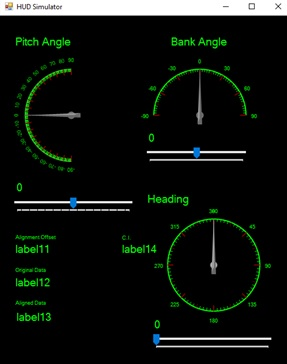
\includegraphics[width=\textwidth,height=\textheight,keepaspectratio]{img/hudsim}
    \label{fig:hudsim}
\end{figure}

\subsection{Remaining Work}
The next step for the user interface is to connect it to the Arduino part of the software. The hardware logistic problem at the beginning of the term has set our team behind the schedule for two weeks. This hinder our team ability to start working on the Arduino portion of the software. Currently, our team is still working on the hardware-software configuration part in Arduino. However, I believe with the current state the user interface, it will take a little time to connect it to the Arduino part of the software. I also would like to do more user study for the graphical user interface. There are significant changes in the user interface and I want to make sure that it still meets the standards of our client. I will start by confirming the user interface to our client this following week.

The next step on the implementation pipeline is the statistical analysis. I am in charged for the statistical analysis for both the pre-aligned data (the original data) and also the aligned data. I am still undecided on which IDE to write my code in. Currently, I am leaning towards to write my code in visual studio since I have been working with the Visual Studio IDE for the user interface. Last term I have done some research for statistical analysis method during the Tech Review. This term, I will start to do more research on the implementation side of the statistical analysis algorithm. The timeline for the statistical analysis portion of the software is tight. Hopefully I can finish the statistical analysis portion of the software on the next two weeks. 

\subsection{Problems and Solutions}
There was a logistical problem at the beginning of the term. Our team were not able to get the hardware required to get started with this project. This problem was frustrating for our team since our project rely heavily with the hardware. Without the hardware it is not possible to get started with the bone and the core of this project. Our hardware is the most important part of the demonstration system. The hardware is where our team get the alignment data as the original data and data to be manipulated with the software.

To solve this problem, our team pro-actively contact the instructor and the TA to get the hardware. Our team sent a bunch of email reminding our instructor to get the hardware. Our team also tried to get in touch with the instructor in person. We came to the instructor office hour to talk about the hardware problem. We also talked about the hardware problem with the TA during meetings to see what our TA can do to help us. Our team also set up a meeting with the clients to let them know about the logistical problem that we were having. The meeting with the clients is important because it eliminates any misunderstanding that might happens between our team and our clients. This pro-active communication has allowed our team to get the necessary hardware faster and maintain our good relationship with the clients. 

The logistical problem that happens at the beginning of the term has set us behind the schedule for 2 weeks. Our team got the necessary hardware at the beginning of week 3 and had to start with the implementation as soon as possible. To save time, our team decided to work in parallel. I was in charge of the graphical user interface portion of the software and my teammates were in charge in the hardware-software configuration. Because our team was working in parallel, everybody can start with their portion of the software. Hence, it saves our team a lot of implementation time. 

At the beginning of the term, I thought that our clients will provide us with the HUD symbology that I can be imported to the graphical user interface. However, this wasn’t the case, our clients have a different method of generating the user interface on the HUD. Our clients used a software that will dynamically generate the HUD display. The Parameters come into the HUD software hosted on a computer via ethernet or Arinc- 429 inputs. Then software draws a distorted picture for the windshield and sent up to the HUD. This is significantly different than what I have in mind. There are no generic HUD symbology that I can directly import to the user interface. Thus, I have to create the HUD display from scratch. 

Creating a HUD display is not an easy task. Rockwell Collins has put a lot of time and energy with their HUD display. Their current HUD display required a sophisticated software to generate it. Hence, creating a full HUD symbology will be out of scope of our project. I tried to be creative and use a gauge to act as the HUD symbology of the user interface. Although the gauge makes the user interface looks more like a car dashboard than an aircraft HUD, the user interface still serve it purpose in describing the data that we will get from our auto alignment system. 

\subsection{Interesting Code}
I use Visual Studio Toolkit to create the graphical user interface of the software. I wrote the code in C to make sure that it is compatible with Arduino. Because our team did not have the Arduino code ready, I decided to use the track bar as a method of debugging the graphical user interface. The track bar can be scrolled side by side to change the value of the gauge in the graphical user interface. To be able to use the gauge icon on the user interface, I imported a dll file called aGauge to my program. 

\begin{lstlisting}[language=c]
		public Form1()
        {
            InitializeComponent();
            label9.Text = "0";
            aGauge3.Value = 0;
            label10.Text = "0";
            aGauge2.Value = 0;
            label8.Text = "0";
            aGauge1.Value = 0;
        }

        private void Form1_Load(object sender, EventArgs e)
        {
            trackBar1.Minimum = -90;
            trackBar1.Maximum = 90;
            trackBar1.TickStyle = TickStyle.BottomRight;
            trackBar1.TickFrequency = 1;
            trackBar3.Minimum = 0;
            trackBar3.Maximum = 360;
            trackBar3.TickStyle = TickStyle.BottomRight;
            trackBar3.TickFrequency = 1;
            trackBar2.Minimum = -90;
            trackBar2.Maximum = 90;
            trackBar2.TickStyle = TickStyle.BottomRight;
            trackBar2.TickFrequency = 1;
        }

        private void trackBar1_Scroll(object sender, EventArgs e)
        {
            label9.Text = trackBar1.Value.ToString();
            aGauge3.Value = trackBar1.Value;
            aGauge3.Refresh();
        }

        private void trackBar2_Scroll(object sender, EventArgs e)
        {
            label8.Text = trackBar2.Value.ToString();
            aGauge1.Value = trackBar2.Value;
            aGauge1.Refresh();
        }

        private void trackBar3_Scroll(object sender, EventArgs e)
        {
            label10.Text = trackBar3.Value.ToString();
            aGauge2.Value = trackBar3.Value;
            aGauge2.Refresh();
        }
\end{lstlisting}

\subsection{First User Study}
I conduct the user study with my friends. Although the graphical user interface doesn’t look like a real HUD from Rockwell Collins, it still serves its purpose. With a little explanation, my friends can grasp the concept and the meaning behind the HUD symbology in the user interface. I used gauge as the HUD symbology of the user interface. At first, it was slightly confusing since it is not a typical flight simulator HUD. My friends told me that it looks more like a car dashboard. I will conduct the user study with our clients next week.  

\begin{figure}
	\centering
 		\caption{The HUD Simulator in Action}
      	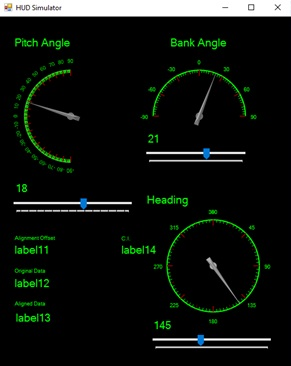
\includegraphics[width=\textwidth,height=\textheight,keepaspectratio]{img/hudsimaction}
    \label{fig:hudsimaction}
\end{figure}





	\input{Drew}

% ============= Conclusion =================
\section{Conclusion}
TODO(D)


\newpage
\nocite{*}
\bibliography{IEEEabrv,References}
\bibliographystyle{IEEEtran}


\end{document}
